\documentclass[a4paper,12pt,oneside]{article}
\usepackage{graphicx}
\usepackage{hyperref}
\usepackage[T1]{fontenc}
\usepackage[utf8]{inputenc}
\usepackage{setspace}
\usepackage{amsmath}
\usepackage{amssymb}

\begin{document}

    \thispagestyle{plain}
    \begin{center}
        \normalsize
        \textbf{Assignment 1}
            
        \vspace{0.2cm}
        \normalsize
        19/10/2022
            
        \vspace{0.2cm}
        \textbf{Francesco Refolli 865955}
    \end{center}

    \section{Esercizio 1}

    \begin{align}
        \text{$max \; x_1 + x_2$} \\
        \text{$x_1 + x_2 \leq 2$} \\
        \text{$2 x_1 - x_2 \leq 0$} \\
        \text{$x_1, x_2 \geq 0$}
    \end{align}

    Costruisco il grafico con le equazioni dei vincoli lungo l'asse $x_1 \times x_2$.
    Riscrivo per comodita' i primi due vincoli in forma equivalente:

    \begin{align}
        \text{$x_1 \leq 2 - x_2$} \\
        \text{$x_1 \leq \frac {x_2} 2$}
    \end{align}

    \begin{center}
        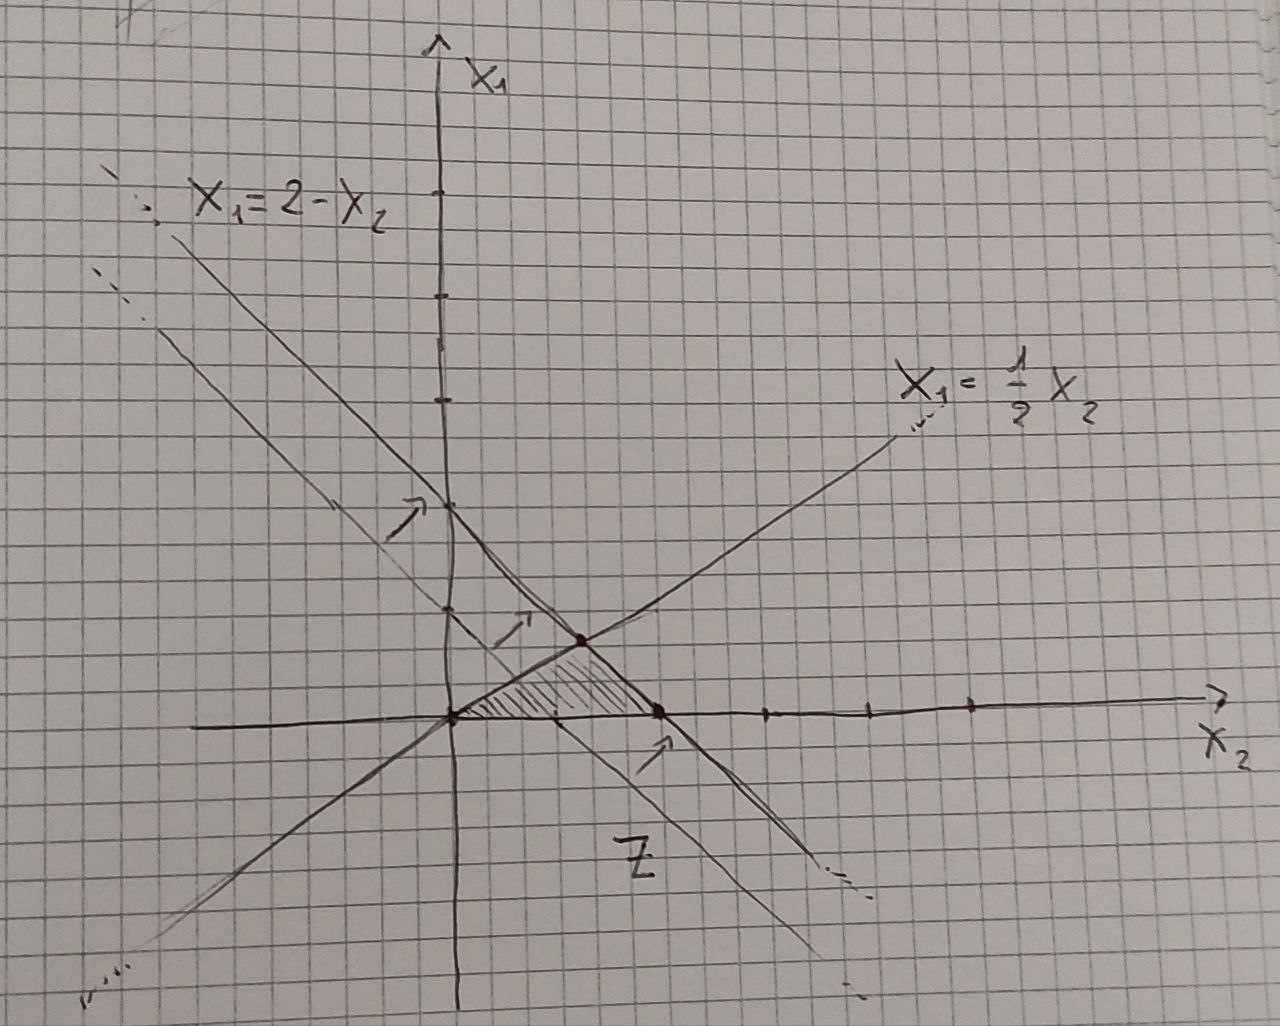
\includegraphics[width=12cm]{grafico.jpg}
    \end{center}

    La direzione di crescita della funzione obiettivo e' perpedincolare al vincolo $x_1 \leq 2 - x_2$, quindi il problema ha \textbf{Infinite Soluzioni Ottime}. \\*
    Le soluzioni sono tutte le coppie <$x_1, x_2$> che risiedono nello spigolo della regione obiettivo su cui si poggia il vincolo $x_1 \leq 2 - x_2$.

    \section{Esercizio 2}

    \begin{align}
        \text{$max \; x_1 + x_2$} \\
        \text{$x_1 + x_2 - x_3 = 2$} \\
        \text{$2 x_1 - x_2 \leq 0$} \\
        \text{$x_1, x_2 \geq 0$} \\
        \text{$x_3 \leq 0$}
    \end{align}

    \paragraph{Conversione in forma standard}

    \subparagraph{1}

    La forma standard non prevede vincoli di non positivita', quindi inverto il segno di $x_3$ in tutti i vincoli:

    \begin{align}
        \text{$max \; x_1 + x_2$} \\
        \text{$x_1 + x_2 + x_3 = 2$} \\
        \text{$2 x_1 - x_2 \leq 0$} \\
        \text{$x_1, x_2, x_3 \geq 0$}
    \end{align}

    \subparagraph{2}

    I vincoli devono essere esclusivamente in forma $\leq$.
    Quindi sostituisco il vincolo $x_1 + x_2 + x_3 = 2$ con l'equivalente in termini di disuguaglianze e inverto il segno di quella con $\geq$.

    \begin{align}
        \text{$max \; x_1 + x_2$} \\
        \text{$x_1 + x_2 + x_3 \leq 2$} \\
        \text{$- x_1 - x_2 - x_3 \leq - 2$} \\
        \text{$2 x_1 - x_2 \leq 0$} \\
        \text{$x_1, x_2, x_3 \geq 0$}
    \end{align}

    \paragraph{Conversione in forma aumentata}

    \subparagraph{1}

    Aggiungo tre variabili di slack per portare i tre vincoli $\leq$ in vincoli $=$.

    \begin{align}
        \text{$max \; x_1 + x_2$} \\
        \text{$x_1 + x_2 + x_3 + x_4 = 2$} \\
        \text{$- x_1 - x_2 - x_3 + x_5 = - 2$} \\
        \text{$2 x_1 - x_2 + x_6 = 0$} \\
        \text{$x_1, x_2, x_3 \geq 0$} \\
        \text{$x_4, x_5, x_6 \geq 0$}
    \end{align}

    \subparagraph{2}

    Quindi esporto la funzione obiettivo $f(x)$ in un vincolo $Z - f(x) = 0$.

    \begin{align}
        \text{$max \; Z$} \\
        \text{$Z - x_1 - x_2 = 0$} \\
        \text{$x_1 + x_2 + x_3 + x_4 = 2$} \\
        \text{$- x_1 - x_2 - x_3 + x_5 = - 2$} \\
        \text{$2 x_1 - x_2 + x_6 = 0$} \\
        \text{$x_1, x_2, x_3 \geq 0$} \\
        \text{$x_4, x_5, x_6 \geq 0$}
    \end{align}

    \paragraph{Risoluzione con tableau}

    \subparagraph{Iterazione 0}

    \begin{center}
        \begin{tabular}{|c|c|c|c|c|c|c|c|c|c|}
            \hline
            base & riga & Z & $x_1$ & $x_2$ & $x_3$ & $x_4$ & $x_5$ & $x_6$ & termine noto \\
            \hline
            Z & 0 & 1 & -1 & -1 &  0 &  0 &  0 &  0 &  0 \\
            $x_4$ & 1 & 0 &  1 &  1 &  1 &  1 &  0 &  0 &  2 \\
            $x_5$ & 2 & 0 & -1 & -1 & -1 &  0 &  1 &  0 & -2 \\
            $x_6$ & 3 & 0 &  2 & -1 &  0 &  0 &  0 &  1 &  0 \\
            \hline
        \end{tabular}
    \end{center}

    \subparagraph{Iterazione 1}

    Sono presenti nella prima riga coefficienti negativi. Seleziono arbitrariamente $x_1$, perche' tutti i coefficienti negativi hanno pari valore. \\

    Nella prima colonna considero i coefficienti delle righe 1, 3. \\*
    Seleziono il minimo rapporto, ovvero 0 della riga 3. \\

    Questo ha l'effetto di togliere dalla base $x_6$ e inserire $x_1$.

    \begin{center}
        \begin{tabular}{|c|c|c|c|c|c|c|c|c|c|}
            \hline
            base & riga & Z & $x_1$ & $x_2$ & $x_3$ & $x_4$ & $x_5$ & $x_6$ & termine noto \\
            \hline
            Z & 0 & 1 &  0 & -$\frac 3 2$ &  0 &  0 &  0 &  $\frac 1 2$ &  0 \\
            $x_4$ & 1 & 0 &  0 &  $\frac 3 2$ &  1 &  1 &  0 & -$\frac 1 2$ &  2 \\
            $x_5$ & 2 & 0 &  0 & -$\frac 3 2$ & -1 &  0 &  1 &  $\frac 1 2$ & -2 \\
            $x_1$ & 3 & 0 &  1 & -$\frac 1 2$ &  0 &  0 &  0 &  $\frac 1 2$ &  0 \\
            \hline
        \end{tabular}
    \end{center}

    \paragraph{Iterazione 2}

    A questo punto seleziono come variabile entrante $x_2$, l'ultima variabile non di base con coefficiente negativo nella prima riga. \\

    Seleziono l'unica riga con coefficiente strettamente positivo, ovvero la riga 1. Quindi $x_4$ esce dalla base. \\

    \begin{center}
        \begin{tabular}{|c|c|c|c|c|c|c|c|c|c|}
            \hline
            base  & riga & Z & $x_1$ & $x_2$        & $x_3$        & $x_4$        & $x_5$ & $x_6$        & termine noto \\
            \hline
            Z     & 0    & 1 &  0    & 0            &  1           &  1           &  0    & 0            & 2 \\
            $x_2$ & 1    & 0 &  0    & 1            &  $\frac 2 3$ &  $\frac 2 3$ &  0    & -$\frac 1 3$ & $\frac 4 3$ \\
            $x_5$ & 2    & 0 &  0    & 0            &  0           &  1           &  1    & 0            &  0 \\
            $x_1$ & 3    & 0 &  1    & 0            &  $\frac 1 3$ &  $\frac 1 3$ &  0    &  $\frac 1 3$ & $\frac 2 3$ \\
            \hline
        \end{tabular}
    \end{center}

    \paragraph{Iterazione 3}

    Non sono piu' presenti coefficienti negativi nella riga 0, quindi l'algoritmo si arresta. \\

    La soluzione ottimale e': \\*
    <$x_1, x_2, x_3, x_4, x_5, x_6$> = <$\frac 2 3, \frac 4 3, 0, 0, 0, 0$> \\

    Visto che le variabili decisionali sono $x_1, x_2$, la soluzione al problema PL e: \\*
    <$x_1, x_2$> = <$\frac 2 3, \frac 4 3$> \\

    \paragraph{1}

\begin{center}
	\begin{tabular}{|c|c|c|c|c|c|c|c|}
		\hline
		Z & $x_1$ & $x_2$ & $x_3$ & $x_4$ & $x_5$ & $x_6$ & b\\
		\hline
		1 & -1 & -1 & 0 & 0 & 0 & 0 & 0\\
		0 & 1 & 1 & 1 & 1 & 0 & 0 & 2\\
		0 & -1 & -1 & -1 & 0 & 1 & 0 & -2\\
		0 & 2 & -1 & 0 & 0 & 0 & 1 & 0\\
		\hline
	\end{tabular}
\end{center}
\begin{center}
	\begin{tabular}{|c|c|c|c|c|c|c|c|}
		\hline
		Z & $x_1$ & $x_2$ & $x_3$ & $x_4$ & $x_5$ & $x_6$ & b\\
		\hline
		1.0 & 0.0 & -1.5 & 0.0 & 0.0 & 0.0 & 0.5 & 0.0\\
		0.0 & 0.0 & 1.5 & 1.0 & 1.0 & 0.0 & -0.5 & 2.0\\
		0.0 & 0.0 & -1.5 & -1.0 & 0.0 & 1.0 & 0.5 & -2.0\\
		0.0 & 1.0 & -0.5 & 0.0 & 0.0 & 0.0 & 0.5 & 0.0\\
		\hline
	\end{tabular}
\end{center}
\begin{center}
	\begin{tabular}{|c|c|c|c|c|c|c|c|}
		\hline
		Z & $x_1$ & $x_2$ & $x_3$ & $x_4$ & $x_5$ & $x_6$ & b\\
		\hline
		1.0 & 0.0 & 0.0 & 1.0 & 1.0 & 0.0 & 0.0 & 2.0\\
		0.0 & 0.0 & 1.0 & $\frac 2 3$ & $\frac 2 3$ & 0.0 & -$\frac 2 3$ & $\frac 4 3$\\
		0.0 & 0.0 & 0.0 & 0.0 & 1.0 & 1.0 & 0.0 & 0.0\\
		0.0 & 1.0 & 0.0 & $\frac 2 3$ & $\frac 2 3$ & 0.0 & $\frac 2 3$ & $\frac 2 3$\\
		\hline
	\end{tabular}
\end{center}

\paragraph{2}

\begin{center}
	\begin{tabular}{|c|c|c|c|c|c|}
		\hline
		Z & $x_1$ & $x_2$ & $x_3$ & $x_4$ & b\\
		\hline
		1 & -1 & -1 & 0 & 0 & 0\\
		0 & 1 & 1 & 1 & 0 & 2\\
		0 & 2 & -1 & 0 & 1 & 0\\
		\hline
	\end{tabular}
\end{center}
\begin{center}
	\begin{tabular}{|c|c|c|c|c|c|}
		\hline
		Z & $x_1$ & $x_2$ & $x_3$ & $x_4$ & b\\
		\hline
		1.0 & 0.0 & -1.5 & 0.0 & 0.5 & 0.0\\
		0.0 & 0.0 & 1.5 & 1.0 & -0.5 & 2.0\\
		0.0 & 1.0 & -0.5 & 0.0 & 0.5 & 0.0\\
		\hline
	\end{tabular}
\end{center}
\begin{center}
	\begin{tabular}{|c|c|c|c|c|c|}
		\hline
		Z & $x_1$ & $x_2$ & $x_3$ & $x_4$ & b\\
		\hline
		1.0 & 0.0 & 0.0 & 1.0 & 0.0 & 2.0\\
		0.0 & 0.0 & 1.0 & $\frac 2 3$ & -$\frac 2 3$ & $\frac 4 3$\\
		0.0 & 1.0 & 0.0 & $\frac 2 3$ & $\frac 2 3$ & $\frac 2 3$\\
		\hline
	\end{tabular}
\end{center}

   
\end{document}
